\begin{center}
\textsc{\Large Laboratorio 12}~\\
{\large Videojuegos, Diseño, Programación}~\\
\emph{Animaciones}
\end{center}

\section{Pre-Laboratorio}
\begin{itemize}
\item Investigar:
\begin{enumerate}
\item Animación por Keyframes.
\item Animación por Motion Capture.
\item Animación Stop-motion
\end{enumerate}
\item Investigar según su herramienta de trabajo como agregar animaciones 2D, 3D. Recomendado probar ejemplos antes del laboratorio.
\item Traer animaciones para integrar en su juego, estas pueden venir desde cualquier fuente que le este disponible.
\end{itemize}

\section{Introducción}
\setlength\intextsep{0pt}
\begin{wrapfigure}[8]{r}{0.2\linewidth}
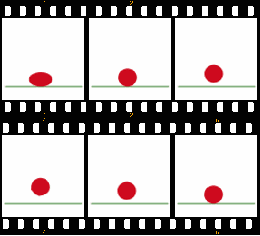
\includegraphics[width=\linewidth]{media/anim_frames.png}
\caption{Cuadros de animación de una pelota rebotando.}
\label{fig:particles}
\end{wrapfigure}
Animación es el proceso de crear la apariencia de movimiento y cambios de forma mostrando rápidamente una secuencia de imágenes estáticas que difieren muy poco entre unas y otras. Los animadores son artistas que se especializan en la creación de animación.

La mayoría de los juegos modernos tienen algún objeto o personaje que necesita ser animado. La excepción en esto esta en juegos de carreras, simuladores o puzzles (e incluso en estos algunos detalles podrían estar animados) \cite[p.~381]{erikgamedevelopment}.
\section{Actividad}
Continuando con el laboratorio anterior durante esta actividad seguimos agregando assets al juego.
\begin{itemize}
\item Durante esta actividad se debe agregar toda clase de assets de arte, texturas, modelos, sonido, etc, se debe remplazar todos los \emph{placeholder} por sus verdaderas representaciones.
\item Debe incluir distintas animaciones a variadas acciones y/o eventos realizados tanto por el jugador principal como por los actores en el mundo de juego.
\item Debe incluir distintas animaciones a variados objetos que considere animados existentes en el mundo de juego.
\item Enlazar eventos y acciones a sonidos y/o efectos visuales que vea necesario.
\end{itemize}
